\setchapterimage[8.5cm]{palomar}
\setchapterpreamble[u]{\margintoc}
\chapter{Transient Follow-up with ZTF}
\labch{ztf_too}
\begin{fquote}[Oscar Wilde][Lady Windermere's Fan][18??]We are all in the gutter, but some of us are looking at the stars
\end{fquote}

The motivation for all real-time analysis and prompt follow-up observations of external triggers is to obtain contemporaneous data. Put another way, these observations are designed to quickly identify time-dependent transient or variable activity which would be missed by untargeted survey operations.  In the case of GW and short GRB follow-up, searches are targeted towards identifying kilonovae (KNe), of which GW170817/AT2017gfo was a spectacular well-documented first example. These KNe are inherently fast-evolving transients which will by definition not be present before the extrenal trigger. For neutrinos, there are a proliferation of possible optical transients (e.g GRBs, TDEs, SNe) and variable objects (primarily blazars) which could be identified in an optical follow-up observations. In both cases, a handful of potentially interesting extragalactic objects will need to be selected against a vast background of spurious detections, and unrelated galactic or solar-system objects.

\section{The Ampel Follow-up Pipeline}
Given the similar challenge, a single flexible analysis, the \ztf, was developed by the author to identify candidate counterparts to GW, GRB and neutrino trigger events. ZTF is particularly well-suited to this type of extragalactic transient discovery,  because ZTF routinely images the visible Northern Sky once every three nights to a median depth of $20.5^{m}$ as part of a public survey \sidecite{ztf_survey_19}.  This provides an extensive base to distinguish between new transients that could be coincident with an external trigger, and those with previous detections. The large volumetric survey speed of ZTF often provides significant serendipitous coverage of events. This wide-field cadence can however be supplemented by dedicated Target-of-Opportunity (ToO) observations scheduled for a particular trigger through the GROWTH ToO Marshal \sidecite{coughlin_19}. 

As introduced in Chapter \ref{ch:ztf}, all ZTF science images are processed, significant detections are extracted, and these are archived in a database at DESY as part of the local computer infrastructure (the \emph{archive database}). External triggers, which come in the form of probability skymaps or GCN circulars, are downloaded and parsed with \ztf. The archive database is then queried for coincident alerts, using either temporal indexing or spatial indexing depending on the size of the target region. Once loaded, these alerts are then filtered by the \ztf~using \emph{AMPEL} \sidecite{ampel}, a platform for realtime analysis of multi-messenger astronomy data. Our selection is based on an algorithm for identifying extragalactic transients \cite{ampel}. In order to identify candidate counterparts, we apply the following cuts to ToO and survey data:

\begin{itemize}
	\item We reject likely subtraction artefacts using machine learning classification and morphology cuts \sidecite{ztf_ml_19}. Subtractions must be positive, i.e a candidate must be brighter than the same position in stacked reference images.
	\item We reject solar system objects through matches to known catalogues \cite{ztf_ml_19}. We further remove uncatalogued solar system objects by requiring multiple detections for each candidate at the same location, separated temporally by at least 15 minutes, thereby rejecting moving objects.
	\item We reject galactic stellar sources by removing detections cross-matched to objects with measured parallax in the second data release of the \emph{GAIA} satellite \sidecite{gaia_dr2}. Objects are rejected if they have non-zero parallax with a significance of at least 3$\sigma$. We further reject likely stars with machine learning classifications, based on sources detected by Pan-STARRS1 \sidecite{ztf_stargalaxy_18}, removing those objects with an estimated stellar probability greater than 80\%. 
	\item We reject AGN variability by cross-matching objects to the WISE survey. We identify likely AGN by applying a series of cuts based on measured IR colour \sidecite{wise_10}.
	\item We rejected unassociated objects by requiring both spatial and temporal coincidence with a given trigger.
\end{itemize}

These cuts typically yield $\sim$0.2 candidates per square degree of sky. Promising candidates are prioritised for spectroscopic classification, to confirm or rule out a possible association with a given neutrino. 

\section{Neutrino Follow-up Program}
ZTF has since its inception had a dedicated program to identify sources of high-energy astrophysical neutrinos, through targeted follow-up observations. A significant component of this thesis was the initial development and operation of this neutrino follow-up program. Given the proliferation of proposed source classes, neutrino follow-up are characterised by searching relatively well-localised regions for poorly-defined objects. This is particularly true for optical follow-up, where potential counterparts include Tidal Disruption Events (TDEs), Type IIn or choked jet SNe, kilonovae, GRB afterglows, superluminous supernovae (SLSNe) or blazar flares (see Chapter \ref{ch:sources} for a comprehensive list). While pre-neutrino detections could rule out neutrino production from choked jet supernovae, in most cases we do not even have stringent constraints in when neutrinos may be expected.

For neutrinos, spatial and temporal coincidence is ensured by requiring that an object lies within the reported 90\% localisation rectangle from IceCube, and being detected at least once following the neutrino arrival time. We have followed up N neutrinos in the period from survey start on 2018 March 20 to 2020 June 31, out of a total of N neutrino alerts published by IceCube. Table \ref{tab:nu_alerts} summarises each neutrino alert that has been observed by ZTF. From 2019 June 17, IceCube published neutrino alerts with improved selection criteria to provide an elevated alert rate \sidecite{ic_realtime_19} (see Chapter \ref{ch:realtime} for more details). In addition to 1 of the 12 alerts under the old V1 selection, ZTF followed up 7 of the 19 alerts published under the V2 selection. In general, we aim to follow all well-localised neutrinos of likely astrophysical origin reported by IceCube which are visible to ZTF and can be observed promptly. 
 
Those alerts not observed by ZTF are summarised in Table \ref{tab:nu_non_observed}. Of those 23 alerts not followed up by ZTF, the primary reasons were proximity to the Sun (8/23), alerts with poor localisation and low astrophysical probability (6/23) and alert retraction (4/23). For events which were reported with estimates of astrophysical probability, we chose not to follow up those that had both low astrophysical probability ($<$ 50\%) and large localisation regions ($>$ 10 sq.\,deg.). This value was not reported for high-energy starting events (HESE) under the old IceCube alert selection, nor for one alert, IC200107A, that was identified outside of the standard alert criteria \sidecite{ic200107a} (see also Chapter \ref{ch:realtime}). The full breakdown of neutrino observations statistics can be seen in Figure N.
 
 Each neutrino localisation region can typically be covered by one or two ZTF observation fields. Multiple observations are scheduled for each field, with both $g$ and $r$ filters, and a separation of at least 15 minutes between images. These observations typically last for 300~s, with a typical limiting magnitude of $21.0^{m}$.  ToO observations are typically conducted on the first two nights following a neutrino alert, before swapping to serendipitous coverage as part of the public survey. 
 
 \begin{figure}[!ht]
 	\centering 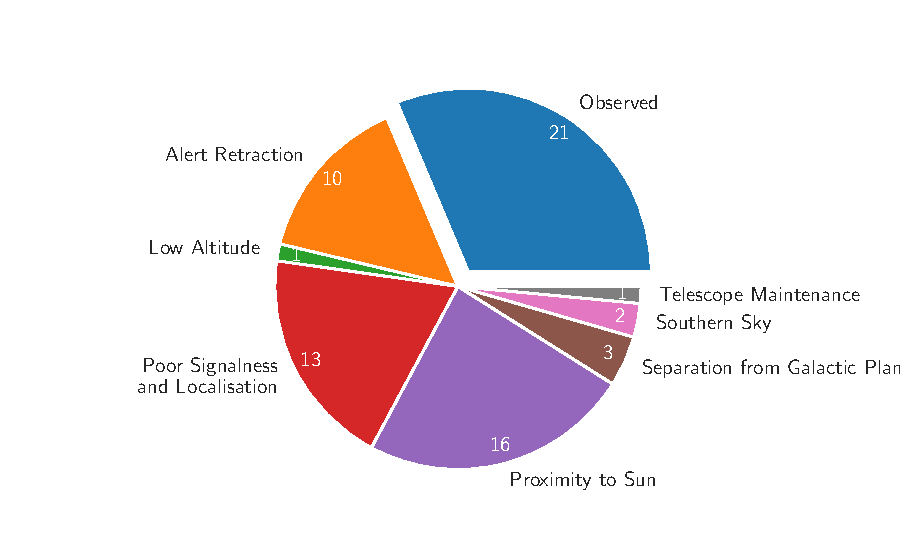
\includegraphics{ztf_too/pie}
 	\caption{Breakdown of the neutrino follow-up program, as of 2021 June 25. }
 	\label{fig:pie}
 \end{figure}
 
 MENTION THAT COMMISSIONING ONE
 
 \begin{table*}
 	\centering
 	\begin{tabular}{||c c c c c c c ||} 
 		\hline
 		\textbf{Event} & \textbf{R.A. (J2000)} & \textbf{Dec (J2000)} & \textbf{90\% area} & \textbf{ZTF obs} &~ \textbf{Signalness}& \textbf{Ref}\\
 		& \textbf{(deg)}&\textbf{(deg)}& \textbf{(sq. deg.)}& \textbf{(sq. deg.)} &&\\
 		\hline
 		IC190503A & 120.28 & +6.35 & 1.94& 1.37 & 36\%&\cite{ic190503a, ic190503a_ztf}\\
 		IC190619A & 343.26 & +10.73 & 27.16& 21.57 & 55\%&\cite{ic190619a, ic190619a_ztf}\\
 		IC190730A & 225.79 & +10.47 & 5.41& 4.52 & 67\%&\cite{ic190730a,ic190730a_ztf}\\
 		IC190922B & 5.76 & -1.57 & 4.48 & 4.09 & 51\%&\cite{ic190922b, ic190922b_atel, ic190922b_ztf}\\
 		\textbf{IC191001A} & \textbf{314.08} & \textbf{+12.94} & \textbf{25.53} & \textbf{20.56} & \textbf{59\%}& \textbf{\cite{ic191001a,ic191001a_atel, ic191001a_ztf}}\\
 		IC200107A & 148.18 & +35.46 & 7.62 & 6.22 & - &\cite{ic200107a,ic200107a_ztf}\\
 		IC200109A & 164.49 & +11.87 & 22.52 & 20.06 & 77\%&\cite{ic200109a,ic200109a_ztf}\\
 		IC200117A & 116.24 & +29.14 & 2.86 &  2.66 & 38\%&\cite{ic200117a,ic200117a_ztf, ic200117a_ztf_2}\\
 		\hline
 	\end{tabular}
 	\caption{Summary of the eight neutrino alerts followed up by ZTF. IC191001A is highlighted in bold. The 90\% area column indicates the region of sky observed at least twice by ZTF, within the reported 90\% localisation, and accounting for chip gaps. The \textit{signalness} estimates the probability that each neutrino is of astrophysical origin, rather than arising from atmospheric backgrounds.}
 	\label{tab:nu_alerts_old}
 \end{table*}

\begin{table*}
	\centering
	\begin{tabular}{||c c c c c c c ||} 
		\hline
		\textbf{Event} & \textbf{R.A. (J2000)} & \textbf{Dec (J2000)} & \textbf{90\% area} & \textbf{ZTF obs} &~ \textbf{Signalness}& \textbf{Ref}\\
		& \textbf{[deg]}&\textbf{[deg]}& \textbf{[sq. deg.]}& \textbf{[sq. deg.]} &&\\
		\hline
		IC190503A & 120.28 & +6.35 & 1.9 & 1.4 & 36\% & \cite{ic190503a, ic190503a_ztf} \\ 
		IC190619A & 343.26 & +10.73 & 27.2 & 21.6 & 55\% & \cite{ic190619a, ic190619a_ztf} \\ 
		IC190730A & 225.79 & +10.47 & 5.4 & 4.5 & 67\% & \cite{ic190730a, ic190730a_ztf} \\ 
		IC190922B & 5.76 & -1.57 & 4.5 & 4.1 & 51\% & \cite{ic190922b, ic190922b_ztf} \\ 
		IC191001A & 314.08 & +12.94 & 25.5 & 20.6 & 59\% & \cite{ic191001a, ic191001a_ztf} \\ 
		IC200107A & 148.18 & +35.46 & 7.6 & 6.2 & - & \cite{ic200107a, ic200107a_ztf} \\ 
		IC200109A & 164.49 & +11.87 & 22.5 & 20.1 & 77\% & \cite{ic200109a, ic200109a_ztf} \\ 
		IC200117A & 116.24 & +29.14 & 2.9 & 2.7 & 38\% & \cite{ic200117a, ic200117a_ztf, ic200117a_ztf2} \\ 
		IC200512A & 295.18 & +15.79 & 9.8 & 9.3 & 32\% & \cite{ic200512a, ic200512a_ztf} \\ 
		IC200530A & 255.37 & +26.61 & 25.3 & 22.0 & 59\% & \cite{ic200530a, ic200530a_ztf, ic200530a_ztf2} \\ 
		IC200620A & 162.11 & +11.95 & 1.7 & 1.2 & 32\% & \cite{ic200620a, ic200620a_ztf} \\ 
		IC200916A & 109.78 & +14.36 & 4.2 & 3.6 & 32\% & \cite{ic200916a, ic200916a_ztf, ic200916a_ztf2} \\ 
		IC200926A & 96.46 & -4.33 & 1.7 & 1.3 & 44\% & \cite{ic200926a, ic200926a_ztf} \\ 
		IC200929A & 29.53 & +3.47 & 1.1 & 0.9 & 47\% & \cite{ic200929a, ic200929a_ztf} \\ 
		IC201007A & 265.17 & +5.34 & 0.6 & 0.5 & 88\% & \cite{ic201007a, ic201007a_ztf} \\ 
		IC201021A & 260.82 & +14.55 & 6.9 & 6.3 & 30\% & \cite{ic201021a, ic201021a_ztf} \\ 
		IC201130A & 30.54 & -12.10 & 5.4 & 4.5 & 15\% & \cite{ic201130a, ic201130a_ztf} \\ 
		IC201209A & 6.86 & -9.25 & 4.7 & 3.2 & 19\% & \cite{ic201209a, ic201209a_ztf} \\ 
		IC201222A & 206.37 & +13.44 & 1.5 & 1.0 & 53\% & \cite{ic201222a, ic201222a_ztf} \\ 
		IC210210A & 206.06 & +4.78 & 2.8 & 2.1 & 65\% & \cite{ic210210a, ic210210a_ztf} \\ 
		IC210510A & 268.42 & +3.81 & 4.0 & 4.0 & 28\% & \cite{ic210510a, ic210510a_ztf} \\ 
		
		\hline
	\end{tabular}
	\caption{Summary of the 21 neutrino alerts followed up by ZTF since survey start on 2018 March 20.}
	\label{tab:nu_alerts}
\end{table*})

 
 \begin{table*}
 	\centering
 	\begin{tabular}{||c c ||} 
 		\hline
 		\textbf{Cause} & \textbf{Events} \\
 		\hline
 		\textbf{Alert Retraction} & IC180423A\cite{ic180423a}, IC181031A\cite{ic181031a}, IC190205A\cite{ic190205a}, IC190529A\cite{ic190529a}\\
 		\hline
 		\textbf{Proximity to Sun} &IC180908A\cite{ic180908a}, IC181014A\cite{ic181014a}, IC190124A\cite{ic190124a}, IC190704A\cite{ic190704a}\\
 		& IC190712A\cite{ic190712a}, IC190819A\cite{ic190819a}, IC191119A\cite{ic191119a}, IC200227A\cite{ic200227a}\\
 		\textbf{Low Altitude} & IC191215A\cite{ic191215a}\\
 		\textbf{Southern Sky} & IC190331A\cite{ic190331a}, IC190504A\cite{ic190504a}\\
 		\hline
 		\textbf{Poor Signalness \& Localisation} &
 		IC190221A\cite{ic190221a}, IC190629A\cite{ic190629a}, IC190922A\cite{ic190922a}\\
 		& IC191122A\cite{ic191122a}, IC191204A\cite{ic191204a}, IC191231A\cite{ic191231a}\\
 		\hline
 		\textbf{Bad Weather} & IC200120A\cite{ic200120a,ic200120a_2}\\
 		\textbf{Telescope Maintenance} & IC181023A\cite{ic181023a}\\
 		\hline
 	\end{tabular}
 	\caption{\textbf{Summary of the 23 neutrino alerts that were not followed up by ZTF since survey start on 2018 March 20.} Of these, 4/23 were retracted, 11/23 were inaccessible to ZTF for various reasons, 6/23 were deemed alerts of poor quality, while just 2/23 were alerts that were missed although they passed our criteria.}
 	\label{tab:nu_non_observed_old}
 \end{table*}

\begin{table*}
	\centering
	\begin{tabular}{||c c ||} 
		\hline
		\textbf{Cause} & \textbf{Events} \\
		\hline
		Alert Retraction & IC180423A \cite{ic180423a}, IC181031A \cite{ic181031a}, IC190205A \cite{ic190205a}, IC190529A \cite{ic190529a} \\ 
		& IC200120A \cite{ic200120a}, IC200728A \cite{ic200728a}, IC201115B \cite{ic201115b}, IC210213A \cite{ic210213a} \\ 
		& IC210322A \cite{ic210322a}, IC210519A \cite{ic210519a} \\ 
		\hline 
		Proximity to Sun & IC180908A \cite{ic180908a}, IC181014A \cite{ic181014a}, IC190124A \cite{ic190124a}, IC190704A \cite{ic190704a} \\ 
		& IC190712A \cite{ic190712a}, IC190819A \cite{ic190819a}, IC191119A \cite{ic191119a}, IC200227A \cite{ic200227a} \\ 
		& IC200421A \cite{ic200421a}, IC200615A \cite{ic200615a}, IC200806A \cite{ic200806a}, IC200921A \cite{ic200921a} \\ 
		& IC200926B \cite{ic200926b}, IC201014A \cite{ic201014a}, IC201115A \cite{ic201115a}, IC201221A \cite{ic201221a} \\ 
		Low Altitude & IC191215A \cite{ic191215a} \\ 
		Southern Sky & IC190331A \cite{ic190331a}, IC190504A \cite{ic190504a} \\ 
		Separation from Galactic Plane & IC201114A \cite{ic201114a}, IC201120A \cite{ic201120a}, IC210516A \cite{ic210516a} \\ 
		\hline 
		Poor Signalness and Localisation & IC190221A \cite{ic190221a}, IC190629A \cite{ic190629a}, IC190922A \cite{ic190922a}, IC191122A \cite{ic191122a} \\ 
		& IC191204A \cite{ic191204a}, IC191231A \cite{ic191231a}, IC200410A \cite{ic200410a}, IC200425A \cite{ic200425a} \\ 
		& IC200523A \cite{ic200523a}, IC200614A \cite{ic200614a}, IC200911A \cite{ic200911a}, IC210503A \cite{ic210503a} \\ 
		& IC210608A \cite{ic210608a} \\ 
		\hline 
		Telescope Maintenance & IC181023A \cite{ic181023a} \\ 
		\hline 
		
	\end{tabular}
	\caption{Summary of the 46 neutrino alerts that were not followed up by ZTF since survey start on 2018 March 20.}
	\label{tab:nu_non_observed}
\end{table*}





%\begin{table*}
%	\centering
%	\begin{tabular}{||c c c c c c c ||} 
%		\hline
%		\textbf{Event} & \textbf{R.A. (J2000)} & \textbf{Dec (J2000)} & \textbf{90\% area} & \textbf{ZTF obs} &~ \textbf{Signalness}& \textbf{Ref}\\
%		& \textbf{(deg)}&\textbf{(deg)}& \textbf{(sq. deg.)}& \textbf{(sq. deg.)} &&\\
%		\hline
%		IC190503A & 120.28 & +6.35 & 1.94& 1.37 & 36\%&\cite{blaufuss:gcn24378,2019ATel12730....1S}\\
%		IC190619A & 343.26 & +10.73 & 27.16& 21.57 & 55\%&\cite{blaufuss:gcn24910, 2019ATel12879....1S}\\
%		IC190730A & 225.79 & +10.47 & 5.41& 4.52 & 67\%&\cite{stein:gcn25225, 2019ATel12967....1T, 2019ATel12974....1S}\\
%		IC190922B & 5.76 & -1.57 & 4.48 & 4.09 & 51\%&\cite{blaufuss:gcn25806,2019ATel13125....1S, stein:gcn25824}\\
%		IC191001A & 314.08 & +12.94 & 25.53 & 20.56 & 59\%& \cite{stein:gcn25913,2019ATel13160....1S, stein:gcn25929}\\
%		IC200107A\footnote{This event was reported without a signalness estimate} & 148.18 & +35.46 & 7.62 & 6.22 & - &\cite{stein:gcn26655,stein:gcn26667}\\
%		IC200109A & 164.49 & +11.87 & 22.52 & 20.06 & 77\%&\cite{stein:gcn26696,reusch:gcn26747}\\
%		IC200117A & 116.24 & +29.14 & 2.86 &  2.66 & 38\%&\cite{lagunas:gcn26802,reusch:gcn26813, reusch:gcn26816}\\
%		IC200512A\footnote{This event occurred at low galactic latitude, and thus our observations were not sensitive to extragalactic objects.}&295.18&+15.79&9.77&9.67&32\%&\cite{IC200512A}\\
%		IC200530A&255.37&+26.61&25.28&22.75&59\%&\cite{IC200530A}\\
%		IC200620A&162.11&+11.95&1.73&1.34&32\%&\cite{IC200620A, ztf_IC200620A}\\
%		\hline
%	\end{tabular}
%	\caption{Summary of the eleven neutrino alerts followed up by ZTF. The 90\% area column indicates the region of sky observed at least twice by ZTF, within the reported 90\% localisation, and accounting for chip gaps. The \textit{signalness} describes the probability that each neutrino is of astrophysical origin, rather than arising from atmospheric backgrounds.}
%	\label{tab:nu_alerts}
%\end{table*}
%
%\begin{table}
%	\centering
%	\begin{tabular}{||c c||} 
%		\hline
%		\textbf{Cause} & \textbf{Events} \\
%		\hline
%		\textbf{Alert Retraction} & IC180423A\cite{IC180423A}, IC181031A\cite{IC181031A},\\ &IC190205A\cite{IC190205A}, IC190529A\cite{IC190529A}\\
%		&\\
%		\hline
%		\textbf{Proximity to Sun} & IC180908A\cite{IC180908A}, IC181014A\cite{IC181014A},\\ &IC190124A\cite{IC190124A}, IC190704A\cite{IC190704A},\\
%		& IC190712A\cite{IC190712A}, IC190819A\cite{IC190819A},\\
%		& IC191119A\cite{IC191119A}, IC200227A\cite{IC200227A}\\
%		&\\
%		\textbf{Low Altitude} & IC191215A\cite{IC191215A}, IC200615A\cite{IC200615A}\\
%		&\\
%		\textbf{Southern Sky} & IC190331A\cite{IC190331A}, IC190504A\cite{IC190504A}\\
%		&\\
%		\hline
%		\textbf{Poor Signalness \& Localisation} &
%		IC190221A\cite{IC190221A}, IC190629A\cite{IC190629A}, \\
%		&IC190922A\cite{IC190922A}, IC191122A\cite{IC191122A}, \\
%		&IC191204A\cite{IC191204A}, IC191231A\cite{IC191231A}\\
%		&IC200410A\cite{IC200410A}, IC200421A\cite{IC200421A}\\
%		& IC200425A\cite{IC200425A}, IC200523A\cite{IC200523A}\\
%		&IC200614A\cite{IC200614A}\\
%		&\\
%		\hline
%		\textbf{Bad Weather} & IC200120A\cite{IC200120A,IC200120A_2}\\
%		&\\
%		\textbf{Telescope Maintenance} & IC181023A\cite{IC181023A}\\
%		&\\
%		\hline
%	\end{tabular}
%	\caption{Summary of the 23 neutrino alerts that were not followed up by ZTF since survey start on 2018 March 20. Of these, 4/23 were retracted, 11/23 were inaccessible to ZTF for various reasons, 6/23 were deemed alerts of poor quality, while just 2/23 were alerts that were missed although they passed our criteria.}
%	\label{tab:nu_non_observed}
%\end{table}
%
%Each neutrino localisation region can typically be covered by one or two ZTF observation fields. Multiple observations are scheduled for each field, with both $g$ and $r$ filters, and a separation of at least 15 minutes between images. These observations typically last for 300~s, with a typical limiting magnitude of $21.0^{m}$.  ToO observations are typically conducted on the first two nights following a neutrino alert, before swapping to serendipitous coverage as part of the public survey. We search ZTF data both preceding and following the arrival of the neutrino. Our coincidence criteria require that an object lie within the 90\% localisation region reported by IceCube in a GCN circular, and must have been detected at least once following the neutrino arrival time. These cuts typically yield $\sim$0.2 candidates per square degree of sky. Promising candidates are prioritised for spectroscopic classification, to confirm or rule out a possible association with a given neutrino. 
%
%A selection of highlighted  results are given below. A further candidate, AT2019dsg, is described in Chapter \ref{ch:bran}.
%
%\subsection{PKS 1502+106}
%As introduced in Chapter \ref{ch:realtime}, the neutrino IC190730A was reported in spatial coincidence with PKS 1502+106, a particularly bright Flat Spectrum Radio Quasar (FSRQ) \sidecite{2019ATel12967....1T}. The object was observed by ZTF as part of ToO observations, and the object DID was also identified by our follow-up pipeline as a candidate counterpart.  The blazar was repeatedly detected as part of the routine survey operations under the name \emph{ZTF18aaqnqzx}, with both positive and negative flux changes relative to survey reference images. The blazar lightcurve is shown in Figure \ref{fig:pks1502_ligtcurve}, with the neutrino arrival time marked in blue. Consistent with observations from other observatories across many wavelengths (Chapter \ref{ch:realtime}), there was no significant flaring observed for this source coincident with the neutrino. The blazar at this point was dimmer than survey reference images, with the neutrino arriving during a year-long fading. 
%
%\begin{figure}[!ht]
%	\centering 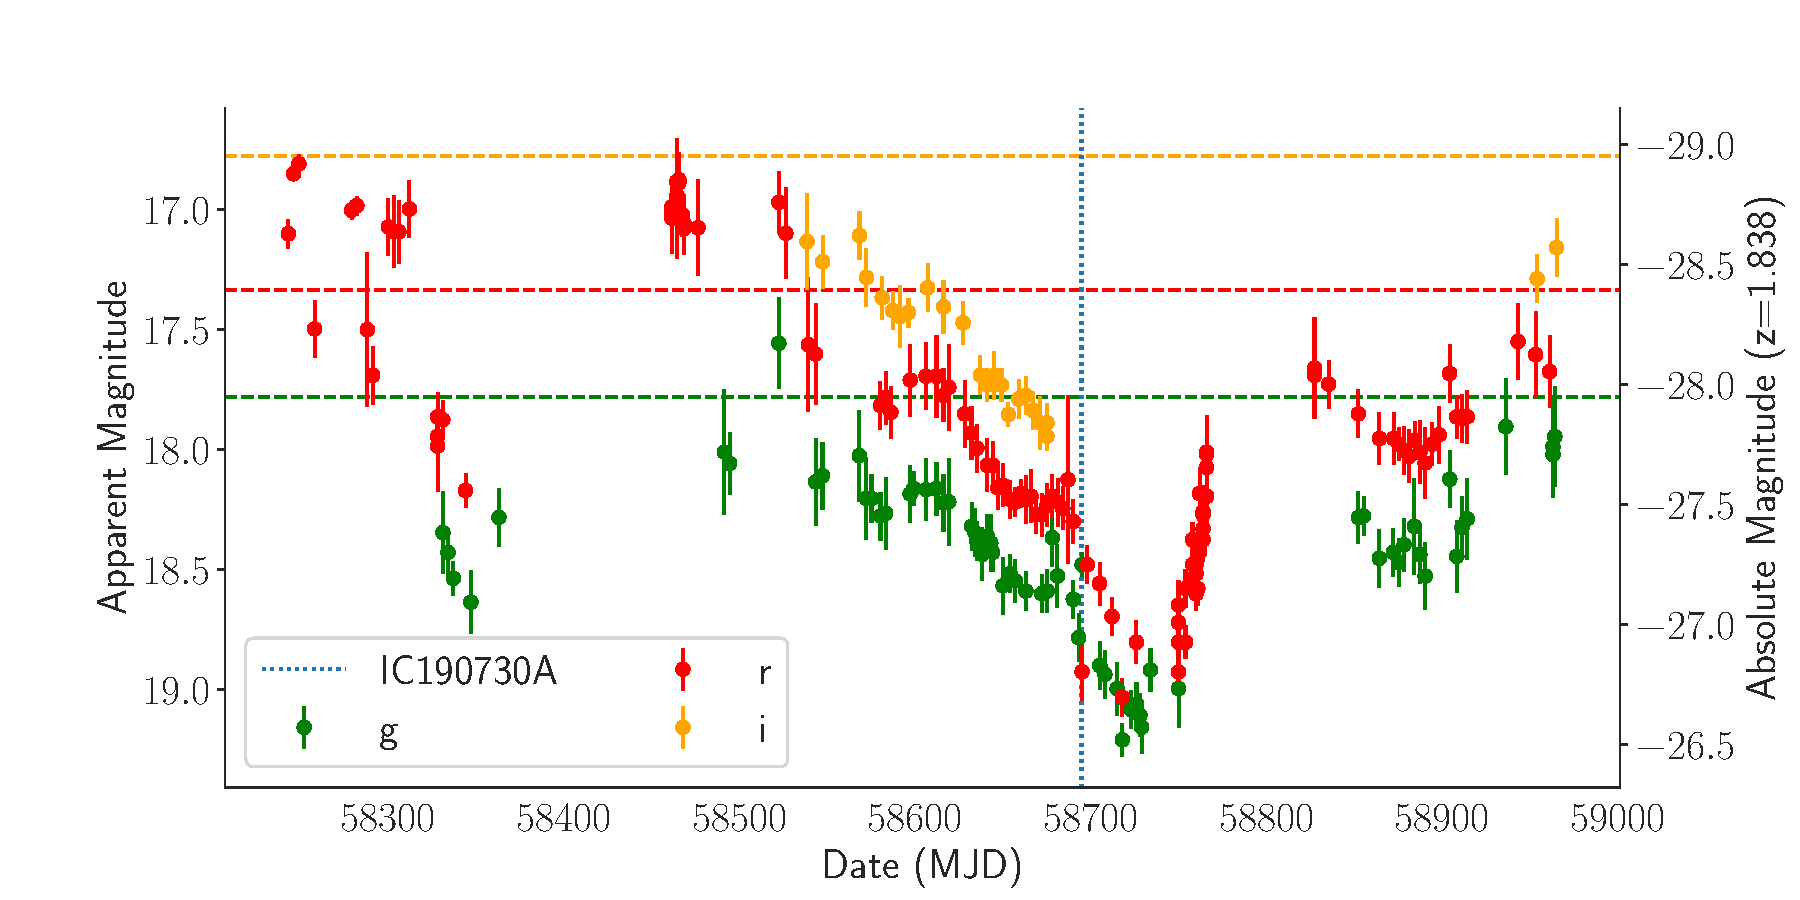
\includegraphics{ZTF/pks1502_lightcurve}
%	\caption{ZTF lightcurve of blazar PKS 1502+106, with observations in g, r and i bands. The arrival time of the neutrino on 2019 July 30 is marked with a dotted line. The horizontal dashed lines indicate the magnitude of the source in reference images derived from the PanSTARRS survey.}
%	\label{fig:pks1502_ligtcurve}
%\end{figure}
%
%\subsection{SN2019pqh}
%As introduced in Chapter \ref{ch:realtime}, follow-up of IC190922B by ZTF identified a candidate supernova ZTF19abxtupj/SN2019pqh \sidecite{2019ATel13125....1S}. As outlined in chapter \ref{ch:sources}, neutrino emission has been predicted for core-collapse supernovae from either choked jets or interacting supernovae. SN2019pqh was not consistent with the former scenario, because it was detected prior to the neutrino. However, it was close to peak, as shown in the lightcurve in Figure \ref{fig:sn2019pqh_ligtcurve}. This was the first young supernova found in coincidence with a high-energy neutrino, which is interesting because CSM neutrino emission . 
%
%\begin{figure}[!ht]
%	\centering 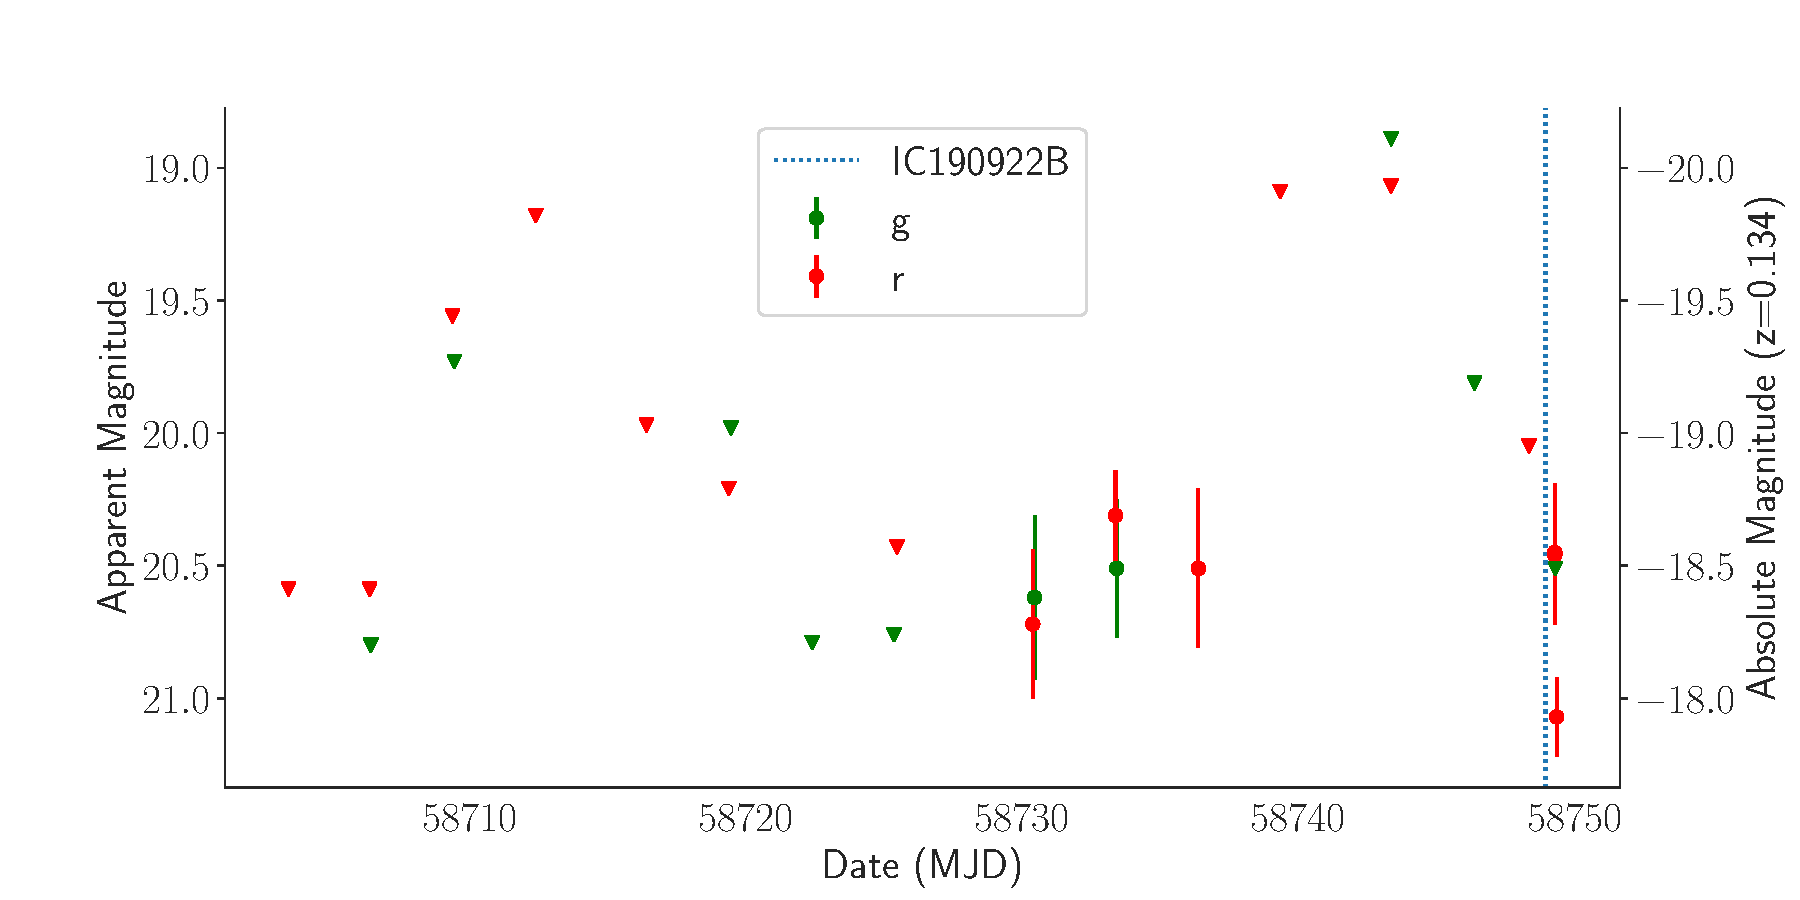
\includegraphics{ZTF/sn2019pqh_lightcurve}
%	\caption{ZTF lightcurve of SN2019pqh, with observations in g and r band. The arrival time of the neutrino on 2019 September 22 is marked with a dotted line, and the supernova is detected in the subsequent ToO obsersations.}
%	\label{fig:sn2019pqh_ligtcurve}
%\end{figure}
%
%This object had first been detected on A subsequent classification of the object as a Type II supernova was reported by ePESSTO (cite). 
%
%A high-resolution spectrum of the object was obtained by De Sharma on 2019 September 28, using the (LRIS) spectrograph at the Keck 1 observatory (see Figure \ref{fig:sn2019pqh_spectrum}). The host galaxy, clearly visible in Figure N, had a spectroscopic redshift of z=0.134 measured by the Sloan .... (SDSS). Peaks are clearly visible in the spectrum matching hydrogen lines for this redshift, confirming that the transient is indeed coincident with the apparent host galaxy.
%
%\begin{figure}[!ht]
%	\centering 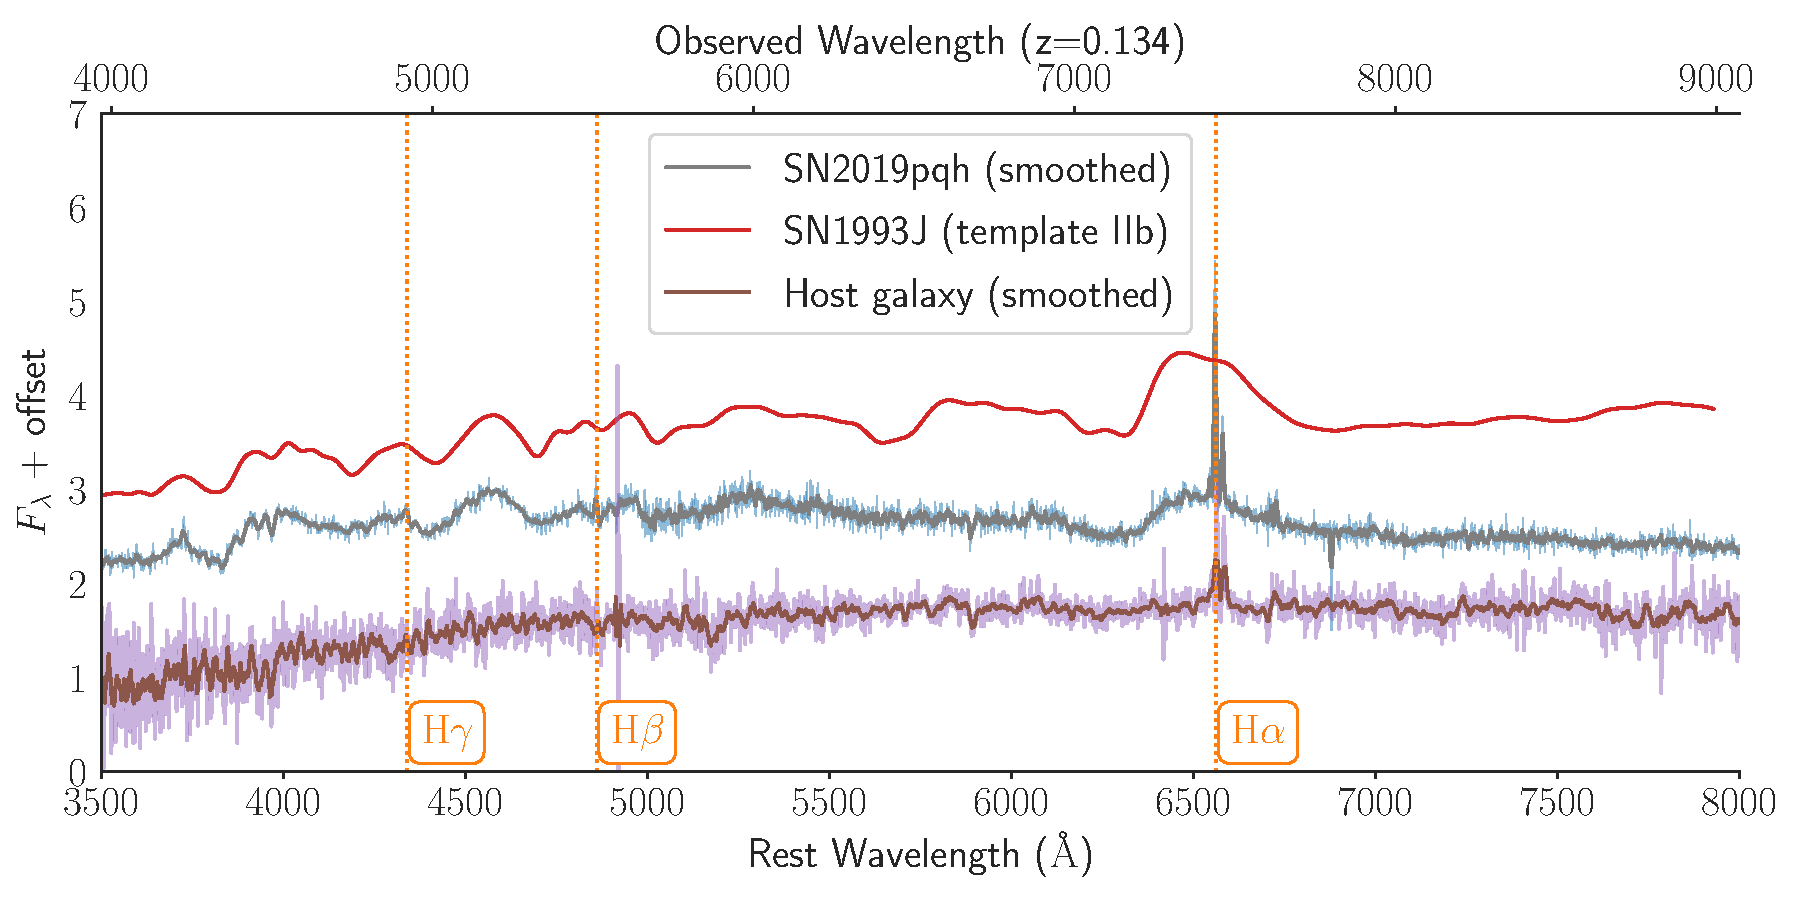
\includegraphics{ZTF/sn2019pqh_spectrum}
%	\caption{Spectrum of SN2019pqh, taken on x. The prominent Balmer lines are highlighted in orange, from which a redshift of 0.134 is derived. A template-matching classification using SNID yields a match to a Type IIb supernova (SN1993J) 2 days before peak cite. }
%	\label{fig:sn2019pqh_spectrum}
%\end{figure}
%
\subsection{AT2019fdr}
\label{sec:at2019fdr}

ZTF serendipitously observed the localisation of neutrino IC200530A just 10 minutes after detection, as part of routine survey operations \sidecite{ic200530a}. Additional ToO observations were then conducted on 2020 May 31 in g- and r-band, and again on 2020 June 1. At this point AT2019fdr was identified by the pipeline as a candidate neutrino source  \sidecite{ic200530a_ztf}. The transient AT2019fdr had originally been discovered by ZTF on 2019 May 03 \cite{at2019fdr_ampel_disc}, but remained in a significantly-elevated flux state at the time of neutrino detection (see Figure \ref{fig:at2019fdr_lightcurve}). 

\begin{figure}[!ht]
	\centering 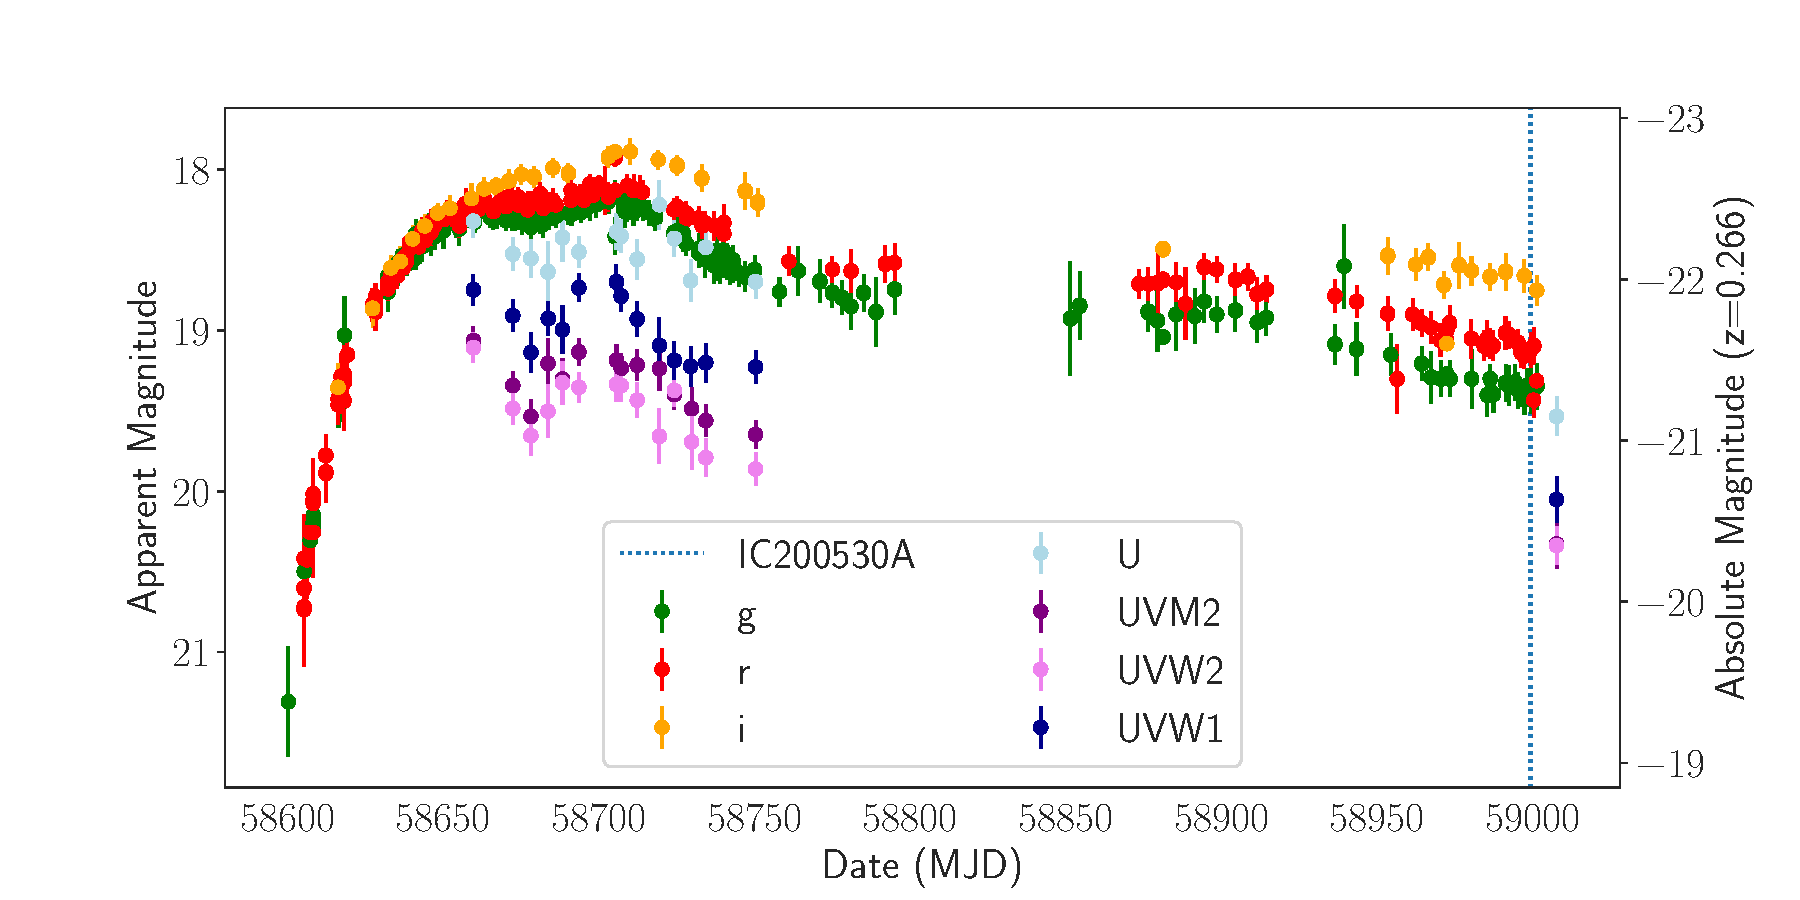
\includegraphics{ZTF/AT2019fdr_lightcurve}
	\caption{ZTF lightcurve of AT2019fdr, with observations in g, r and i band. }
	\label{fig:at2019fdr_lightcurve}
\end{figure}

A spectrum of the object was taken on 2019 June 8, which gave an ambiguous classification but found a redshift of 0.267 on the basis of nebular emission lines (see Figure \ref{fig:at2019fdr_spectra}). Given the consistency of the transient position with the host nucleus, and the bright nature of transient, there was initially considerable interest in this object as a possible TDE or superluminous supernova (SLSN). As can be seen in Figure \ref{fig:at2019fdr_lightcurve}, the transient peaked at an absolute magnitude of -22.8 in i-band, with little apparent fading through to the detection of the neutrino 10 months later. 

\begin{figure}[!ht]
	\centering 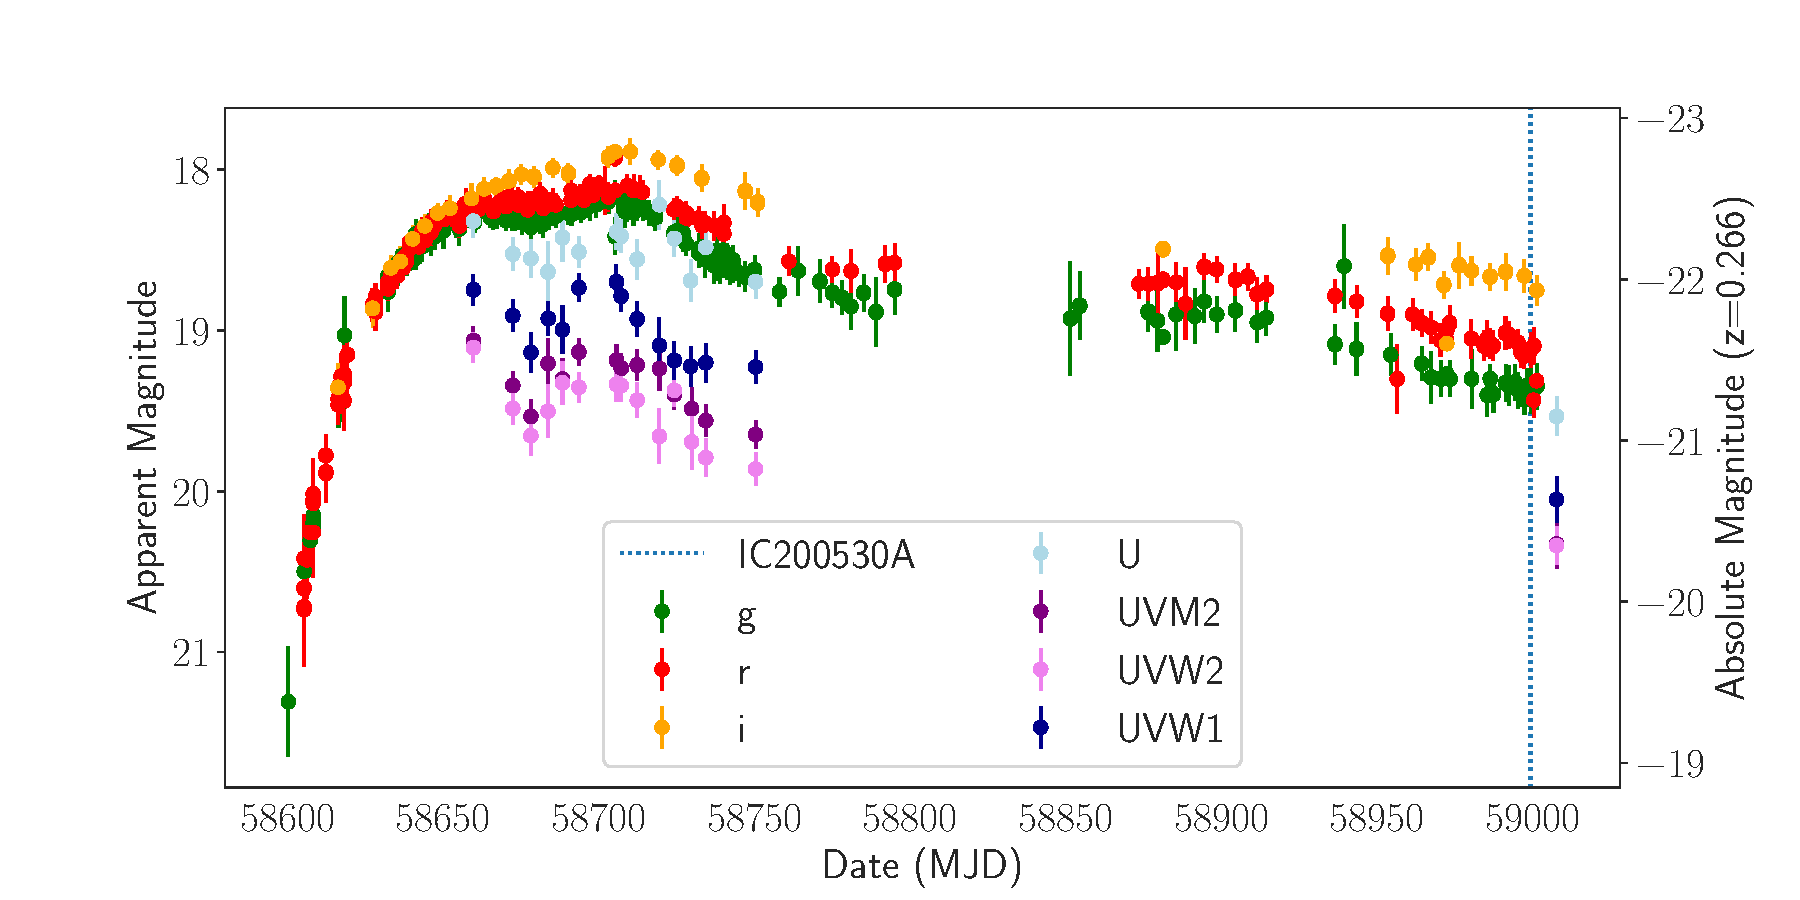
\includegraphics{ZTF/AT2019fdr_lightcurve}
	\caption{ZTF lightcurve of AT2019fdr, with observations in g, r and i band. }
	\label{fig:at2019fdr_spectra}
\end{figure}

The object was tentatively classified as a luminous Type IIn supernova, though the possibility of an AGN classification was also mentioned \cite{at2019fdr_tns_class}. Given the lack of temperature evolution over the subsequent 10 months of observation, a supernova classification seems unlikely. Instead, AT2019fdr more likely belongs to a recently-identified class of flares in Narrow-line Seyfert galaxies \sidecite{trakhtenbrot19}. Indeed, our late-time spectroscopy (Figure \ref{fig:at2019fdr_spectra}) reveals iron emission lines  characteristic of these flares.

Flares that fall into the spectroscopic class defined by \sidecite{trakhtenbrot19} all occurred in Narrow-Line Seyfert\,1 (NLS1) galaxies. They show a large long-duration flare which leads to a sustained flux increase on timescales of many months, with little apparent temperature or color evolution. Such flares also have characteristic spectroscopic features, namely emission lines at $\lambda4640$ and $\lambda4686$ as well as an OIII-complex, which distinguish them from other objects. These signatures are also present for AT2019fdr (red and blue lines in Figure \ref{fig:at2019fdr_spectra}).

To date, ZTF has identified 5 large outburst from NLS1's. Accounting for all neutrinos followed-up by ZTF, \textbf{the probability that such a flare should be found by chance is just 0.9\%}. It is thus likely that AT2019fdr is indeed the source of IC200530A. AT2019fdr is the first NLS1 flare reported in spatial and temporal coincidence with a high-energy neutrino. However, neutrino emission has been predicted theoretically from Seyfert galaxies \cite[see e.g]{murase_agn}. Indeed, in light of AT2019dsg, recent theoretical work has suggested that tidal disruption events may share a common neutrino production mechanism with active galaxy cores \sidecite{murase_bran}. 

Observations of AT2019fdr contemporaneous with the neutrino detection are needed to enable comprehensive modelling of the object, and identify possible mechanisms for neutrino production. Radio observations could again reveal the presence of an outflow, found for AT2019dsg and independently proposed for these flares \cite{trakhtenbrot19}. Such outflows may indeed be the key signature of neutrino production. Conversely, a radio non-detection would strongly disfavour the association of this object with IC200530A.
%
\subsection{SN2020xxx}

Two likely supernovae were also identified by the pipeline \cite{ic200530a_ztf}, but this is compatible with background expectations, and one has since been firmly excluded as a neutrino counterpart through spectroscopic classification. The other...

\subsection{SN2019pqh}
\label{sec:sn2019pqh}

\section{Gravitational Waves and Gamma-ray Bursts}
In contrast to neutrinos, follow-up of GW and GRB triggers is more akin to searching for a needle in a haystack. The localisations tend to be much larger than for neutrinos, but with the well-defined aim of finding kilonovae. In this case, we at least know what our needle looks like. GW170817 provided an observational confirmation of theoretical predictions of kilonovae, namely that they are faint, fast-evolving, red transients which are generated following mergers of neutron stars. Though a trigger event may cover several hundred or thousand square degrees, these constraints enable us to efficiently reject the vast majority of candidates. Additional temporal coincidence is ensured by requiring that candidates are not detected prior to merger/burst, and spatial coincidence can be ensured using trigger probability skymaps integrated out to predefined confidence intervals (typically 90\% or 95\%). Unique among triggers, GW events are also typically reported with estimated distance ranges derived from template-matching. For candidates which have a resolved host galaxy, we can determine their distance using spectroscopic surveys such as SDSS, as well as photometric redshift estimates, and veto those candidates lying outside the desired distance range.

The third observing run of the LIGO/VIRGO (O3) extended from X to y, and for this period ZTF has followed-up LVc GW triggers. In this period, there were BNs candidates and Y BBH candidates.

There have been some predictions of EM signatures for BBH events...

\begin{table*}
	\centering
	\begin{tabular}{||c c c c c c c c c c||} 
		\hline
		\textbf{Name} & \textbf{P$_{\textup{t}}$} & \textbf{Area} & \textbf{Distance} & \textbf{Class} & \textbf{P$_{\textup{1}}$} & \textbf{P$_{\textup{2}}$} & \textbf{Time Lag} & \textbf{Depth} & \textbf{E(B$-$V)}\\
		&&(sq. deg.)&(Mpc)&&&&(hr)&&\\
		\hline
		GW190425 &  1\% & 7461  & 156 $\pm$ 41& BNS & 24.13\%  & 23.90\%  & 0.003& 21.5 & 0.03\\
		S190426c & 58\% & 1131  & 377 $\pm$ 100 & NSBH & 52.33\%  & 51.57\% & 13.06& 21.5 & 0.34\\
		S190814bv & 1\% & 23  & 267 $\pm$ 52 & NSBH & 88.57 \%  &  78.37\%  & 0.00 & 21.0 & 0.02\\ % check this
		S190901ap & 14\% & 14753  & 241 $\pm$ 79  & BNS & 56.94\% & 49.39\%  & 3.61& 21.0 & 0.03\\
		S190910d & 2\% & 2482 & 632 $\pm$ 186  & NSBH & 32.99\% & 31.17\%& 1.51& 20.3 & 0.04\\
		S190910h & 39\% & 24264 & 230 $\pm$ 88 & BNS & 33.26\%  & 28.92\% & 0.015& 20.4 & 0.08\\
		S190923y & 32\% & 2107  & 438 $\pm$ 133& NSBH & 38.99\%  & 19.22\% & 13.73& 20.1 & 0.09\\
		S190930t & 26\% & 24220  & 108 $\pm$ 38 & NSBH & 50.63\% & 43.42\% & 11.91& 21.1 & 0.05\\
		S191205ah & 7\% & 6378  & 385 $\pm$ 164  & NSBH & 5.68\% & 4.85\% & 10.66& 17.9 & 0.04\\
		S191213g & 23\% & 4480 & 201 $\pm$ 81  & BNS & 27.50\%  & 25.10\% & 0.013& 20.4 & 0.30\\
		S200105ae & 97\%& 7373  & 283 $\pm$ 74  & NSBH & 52.39\% & 43.99\%  & 9.96 & 20.2 & 0.05\\
		S200115j & 1\% & 765 & 340 $\pm$ 79 & NSBH & 22.21\% & 15.76\%  & 0.24 & 20.8 & 0.13\\
		S200213t & 37\% & 2326  & 201 $\pm$ 80& BNS & 72.17\% & 70.48\%  & 0.40 & 21.2 & 0.19\\
		\hline
	\end{tabular}
	\caption{Summary of ZTF follow-up of 13 gravitational wave events in O3. We list the GW False Alarm Rate (FAR) and in parantheses, the probability that the event is terrestrial (P$_{\textup{t}}$). We list the total size of the GW localization region, the GW median distance and the most probable GW classification. We report the integrated probability within the 90\% contour of the LALinference skymap, covered by triggered and serendipitous ZTF searches during the first three days after merger observed at least once (P$_{\textup{1}}$), and probability observed at least twice (P$_{\textup{2}}$). In parentheses, we include the coverage based on the BAYESTAR skymap. For some events, only BAYESTAR skymaps were made available. All estimates correct for chip gaps and processing failures. We also report the time lag between merger time and start of ZTF observations (hours), the median depth (AB mag), and the median line-of-sight extinction.}
	\label{tab:gw_alerts}
\end{table*}
